\documentclass[10pt]{article}

\usepackage[margin=0.68in]{geometry}
\usepackage[numbers,sort&compress]{natbib}
\usepackage{xurl}
\usepackage[colorlinks=true,linkcolor=blue,citecolor=blue,urlcolor=blue]{hyperref}
\usepackage{amsmath}
\usepackage{booktabs}
\usepackage{array}
\usepackage{graphicx}
\usepackage{tikz}
\usetikzlibrary{arrows.meta,positioning,shapes.geometric}

\setlength{\parindent}{0pt}
\setlength{\parskip}{2.8pt}
\emergencystretch=2em
\renewcommand{\refname}{Referensi}
\renewcommand{\figurename}{Gambar}
\renewcommand{\tablename}{Tabel}
\renewcommand{\abstractname}{Abstrak}

\title{\textbf{Simulasi Adaptasi Agen melalui Reinforcement Learning dan Seleksi Alam}}
\author{
Muhammad Fathur Rizky (13523105)\\
Reza Ahmad Syarif (13523119)\\
Guntara Hambali (13523114)\\
Muh Rusmin Nurwadin (13523068)
}
\date{}

\begin{document}
\maketitle

\begin{abstract}
Penelitian ini mengevaluasi simulasi evolusi agen yang menggabungkan pembelajaran individual berbasis Q-learning dengan seleksi alam antargenerasi. Simulasi diformulasikan dengan pendekatan Markov Decision Process dalam kerangka agent-based modeling, yaitu agen mencari makanan, menghindari bahaya, mengelola energi, bereproduksi, dan mewariskan sifat \textit{speed}, \textit{endurance}, \textit{foraging}, serta \textit{reproduction}. Eksperimen mandiri dilakukan pada tujuh skenario, masing-masing tiga seed, selama 12 generasi dan 260 langkah per generasi. Hasil menunjukkan bahwa baseline mencapai fitness akhir rata-rata 94,06, eksplorasi tinggi mencapai 100,04, dan hazard rendah mencapai 96,75. Hazard tinggi menurunkan fitness menjadi 70,12, sedangkan mutasi rendah menghasilkan kenaikan fitness paling kecil, yaitu 1,66. Temuan ini menunjukkan bahwa adaptasi terbaik tidak cukup dibaca dari fitness akhir, tetapi dari keseimbangan antara eksplorasi perilaku, variasi genetik, tekanan seleksi, stabilitas antar-seed, dan biaya ekologis. Selain itu, dapat disimpulkan bahwa penelitian ini berhasil menyimulasikan seleksi alam melalui algoritma Q-learning.
\end{abstract}

\section{Pendahuluan}
Evolusi biologis menjelaskan perubahan sifat populasi melalui variasi, pewarisan, dan reproduksi diferensial \citep{darwin1859origin}. Dalam komputasi evolusioner, prinsip tersebut disimulasikan melalui populasi kandidat, evaluasi fitness, seleksi, crossover, dan mutasi \citep{holland1992adaptation,mitchell1998introduction}. Penelitian ini memodelkan prinsip yang sama pada agen buatan, yaitu variation muncul dari mutasi sifat dan nilai Q, inheritance muncul dari pewarisan trait dan sebagian Q-table, sedangkan differential reproduction muncul dari fitness-proportionate selection.

Reinforcement learning (RL) mempelajari kebijakan tindakan dari interaksi berulang antara agen dan lingkungan \citep{sutton2018reinforcement}. Secara formal, simulasi dapat dipandang sebagai aproksimasi Markov Decision Process (MDP), $\mathcal{M}=(\mathcal{S},\mathcal{A},P,R,\gamma)$, dengan state, aksi, transisi, reward, dan discount factor. Q-learning dipilih karena merupakan metode temporal-difference off-policy yang memperbarui nilai pasangan state--aksi berdasarkan reward langsung dan nilai maksimum state berikutnya \citep{watkins1992q}. Dalam penelitian ini, RL merepresentasikan adaptasi perilaku dalam masa hidup agen, sedangkan seleksi dan mutasi merepresentasikan perubahan populasi lintas generasi.

Simulasi ini juga merupakan agent-based model. Setiap agen memiliki posisi, energi, sifat biologis, Q-table, dan aturan interaksi dengan makanan, bahaya, serta agen lain. Pendekatan berbasis agen cocok karena fenomena makro seperti fitness rata-rata, survival rate, reproduksi, dan distribusi sifat muncul dari aturan mikro yang sederhana \citep{gilbert2008agent}. Kerangka Gymnasium membantu menjaga pemisahan antara observasi, aksi, reward, dan terminasi episode \citep{towers2024gymnasium}.

Hubungan antara pembelajaran individual dan evolusi populasi dapat dilihat melalui Baldwin effect, yaitu teori yang menyatakan bahwa kemampuan belajar dapat mengubah arah seleksi karena individu yang mampu belajar perilaku adaptif memperoleh fitness lebih tinggi \citep{baldwin1896new,downing2012baldwin}. Model ini tidak mengklaim membuktikan Baldwin effect secara biologis, tetapi memakai gagasan tersebut sebagai hipotesis simulasi, yaitu Q-learning meningkatkan perilaku selama hidup agen, lalu fitness yang dihasilkan memengaruhi peluang agen menjadi induk.

Pertanyaan penelitian yang dikaji adalah, \textit{bagaimana Q-learning dapat menyimulasikan adaptasi agen di bawah tekanan seleksi alam, dan bagaimana perubahan parameter mutasi, bahaya, serta eksplorasi memengaruhi fitness dan sifat populasi?} Tujuan penelitian ini adalah menyusun eksperimen terukur untuk menilai kontribusi pembelajaran perilaku dan seleksi alam dalam dinamika populasi buatan. Kontribusinya adalah kerangka evaluasi yang dapat dijalankan ulang, dilengkapi metrik kuantitatif dan interpretasi biologis.

\section{Metode}
Model penelitian terdiri atas empat komponen utama, yaitu populasi agen adaptif, lingkungan dua dimensi dengan makanan dan bahaya, mekanisme pembelajaran perilaku berbasis Q-learning, serta mekanisme evolusi berupa seleksi induk, crossover, dan mutasi. Simulasi dijalankan sebagai eksperimen komputasional berulang sehingga perubahan fitness, survival, reproduksi, dan sifat populasi dapat diamati lintas generasi.

Setiap agen memiliki empat sifat. \textit{Speed} meningkatkan jarak gerak, tetapi menaikkan biaya metabolisme. \textit{Endurance} menurunkan biaya gerak dan dampak bahaya. \textit{Foraging} meningkatkan efektivitas pengambilan makanan. \textit{Reproduction} menaikkan peluang reproduksi ketika dua agen cukup dekat dan memiliki energi memadai.

Lingkungan berbentuk bidang dua dimensi berukuran 100 x 72. Makanan disebar secara acak dan diganti setiap kali berhasil dikonsumsi, sedangkan zona bahaya berbentuk lingkaran dengan radius tertentu. Agen kehilangan energi akibat metabolisme dan pergerakan. Ketika berada dalam zona bahaya, energi agen berkurang lebih besar, sedangkan ketika mencapai makanan, energi bertambah sesuai kemampuan foraging. Agen mati apabila energi habis atau umur melewati batas maksimum. Dengan demikian, setiap tindakan memiliki konsekuensi, misalnya bergerak dapat mendekatkan agen ke makanan atau pasangan, tetapi juga menghabiskan energi dan dapat membawa agen ke zona berbahaya.

State agen didiskretisasi menjadi 10 komponen, yaitu posisi $x$ dan $y$, arah dan jarak makanan terdekat, arah dan jarak bahaya terdekat, energi, dan umur. Aksi terdiri atas bergerak ke atas, bawah, kiri, kanan, diam, dan mencari pasangan reproduksi. Model Q-learning menggunakan aturan
\[
Q(s,a) \leftarrow Q(s,a) + \alpha \left(r + \gamma \max_{a'}Q(s',a') - Q(s,a)\right),
\]
dengan $\alpha=0{,}22$, $\gamma=0{,}92$, dan $\epsilon=0{,}18$ pada baseline. Reward positif diberikan untuk bertahan hidup, memakan makanan, dan reproduksi berhasil, sementara reward negatif diberikan untuk bahaya, kegagalan reproduksi, biaya pencarian pasangan, dan kematian.

Metode tabular lain yang relevan sebagai pembanding adalah SARSA dan Expected SARSA \citep{sutton2018reinforcement}. SARSA bersifat on-policy karena memperbarui nilai berdasarkan aksi aktual $a'$ yang dipilih policy,
\[
Q(s,a) \leftarrow Q(s,a)+\alpha\left(r+\gamma Q(s',a')-Q(s,a)\right),
\]
sedangkan Expected SARSA memakai ekspektasi terhadap semua aksi berikutnya, $\sum_{a'}\pi(a'|s')Q(s',a')$. Keduanya cocok untuk eksperimen lanjutan, terutama pada hazard tinggi, karena dapat menguji apakah metode on-policy menghasilkan perilaku lebih konservatif daripada Q-learning yang off-policy.

Secara ringkas, state dan aksi dapat ditulis sebagai
\[
s_t=(x_b,y_b,d^x_f,d^y_f,\rho_f,d^x_h,d^y_h,\rho_h,e_b,a_b), \qquad
\mathcal{A}=\{\uparrow,\downarrow,\leftarrow,\rightarrow,\mathrm{diam},\mathrm{reproduksi}\}.
\]
Kebijakan $\epsilon$-greedy yang digunakan agen adalah
\[
\pi(a|s)=
\begin{cases}
1-\epsilon+\epsilon/|\mathcal{A}|, & a=\arg\max_{a'}Q(s,a'),\\
\epsilon/|\mathcal{A}|, & \text{lainnya}.
\end{cases}
\]

Representasi state tersebut adalah aproksimasi Markov, bukan representasi sempurna dari seluruh dunia. Agen tidak menyimpan riwayat lintasan, posisi semua agen lain, atau konfigurasi lengkap semua makanan dan bahaya. Asumsi yang digunakan adalah bahwa ringkasan posisi relatif, energi, dan umur cukup informatif untuk menghasilkan kebijakan adaptif. Konsekuensinya, hasil Q-learning harus diinterpretasikan sebagai performa pada state diskret yang terbatas. Diskretisasi yang lebih kasar dapat menghilangkan informasi, sedangkan diskretisasi yang lebih halus dapat memperbesar Q-table dan memperlambat pembelajaran.

Nilai eksplorasi mengalami peluruhan antargenerasi sampai batas minimum pada konfigurasi baku. Mekanisme ini penting karena agen tidak mengetahui lokasi makanan, bahaya, atau pasangan secara sempurna, tetapi hanya menerima state diskret yang merangkum kondisi lokal relatif.

Fitness dihitung dari total reward, umur, makanan, reproduksi, bahaya, dan status hidup, yaitu
\[
F = R + 0{,}09A + 9{,}5M + 22B - 4H + L,
\]
dengan $R$ total reward, $A$ umur, $M$ jumlah makanan, $B$ jumlah reproduksi, $H$ paparan bahaya, dan $L=12$ jika agen masih hidup. Seleksi induk menggunakan fitness-proportionate selection dengan tekanan seleksi 1,35. Anak mewarisi rata-rata sifat dua induk, mengalami mutasi, dan menerima Q-table hasil crossover serta mutasi nilai Q.

Probabilitas agen $i$ dipilih sebagai induk adalah
\[
p_i=\frac{F_i^\tau}{\sum_j F_j^\tau}, \qquad \tau=1{,}35,
\]
sedangkan mutasi trait anak dimodelkan sebagai
\[
z_{\mathrm{anak}}=\mathrm{clip}\!\left(\frac{z_1+z_2}{2}+\eta,\;z_{\min},z_{\max}\right), \quad
\eta\sim \begin{cases}\mathcal{N}(0,\sigma_z^2),& u<\mu,\\0,&u\geq\mu,\end{cases}
\]
dengan $\mu$ laju mutasi dan $z$ salah satu trait biologis.

Dalam proses reproduksi, dua agen harus sama-sama hidup, memiliki energi di atas ambang reproduksi, dan berada dalam radius reproduksi. Apabila syarat ini terpenuhi, peluang keberhasilan ditentukan oleh rata-rata sifat \textit{reproduction} kedua agen. Reproduksi mengurangi energi induk, tetapi menambah individu baru. Pada akhir generasi, populasi berikutnya dibentuk melalui seleksi induk berdasarkan fitness. Hal ini membedakan kelahiran langsung dalam episode dari regenerasi populasi antar generasi.

Untuk dua agen yang memenuhi syarat jarak dan energi, peluang reproduksi ditulis sebagai
\[
P(\mathrm{reproduksi}\mid i,j)=\frac{r_i+r_j}{2},
\]
dengan $r_i$ dan $r_j$ nilai trait \textit{reproduction}.

Terdapat empat asumsi model yang penting. Pertama, genotipe disederhanakan menjadi empat trait numerik. Kedua, fitness adalah aproksimasi komputasional, bukan fitness biologis murni. Ketiga, lingkungan tidak merepresentasikan organisme atau ekosistem tertentu. Keempat, pewarisan Q-table adalah asumsi komputasional, yaitu keturunan menerima sebagian pengalaman induk melalui crossover nilai Q. Asumsi terakhir sengaja dipakai untuk menguji interaksi learning--evolution, tetapi tidak boleh dibaca sebagai analogi biologis langsung terhadap pewarisan pengalaman.

\begin{figure}[h]
\centering
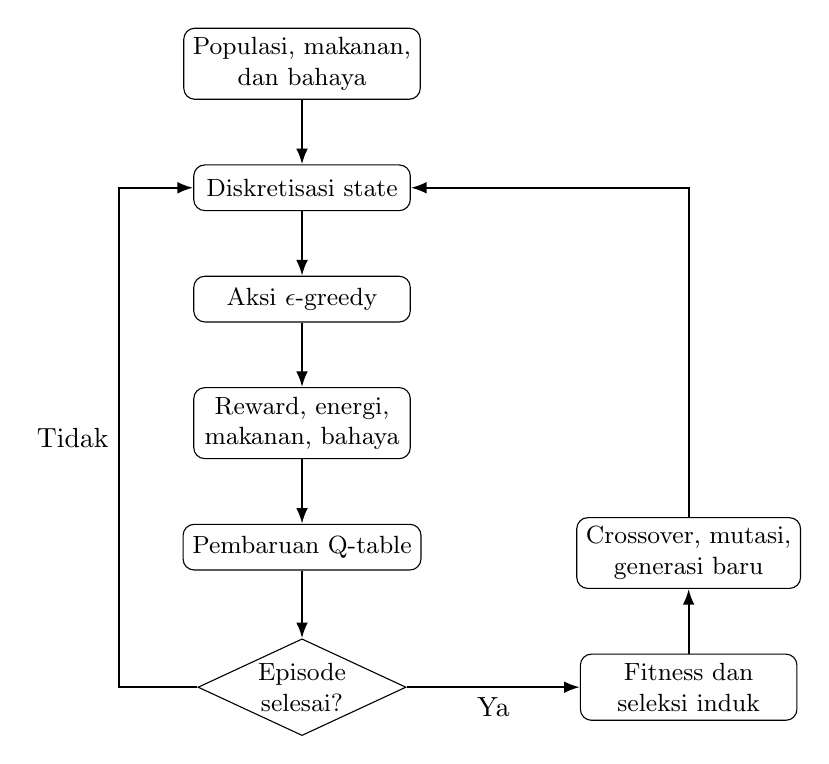
\begin{tikzpicture}[
  node distance=0.82cm,
  box/.style={rectangle,draw,rounded corners,align=center,minimum width=2.75cm,minimum height=0.58cm,font=\small},
  decision/.style={diamond,draw,aspect=2.15,align=center,inner sep=1pt,font=\small},
  arrow/.style={-{Latex[length=2mm]},thick}
]
\node[box] (init) {Populasi, makanan,\\dan bahaya};
\node[box,below=of init] (state) {Diskretisasi state};
\node[box,below=of state] (act) {Aksi $\epsilon$-greedy};
\node[box,below=of act] (env) {Reward, energi,\\makanan, bahaya};
\node[box,below=of env] (update) {Pembaruan Q-table};
\node[decision,below=of update,yshift=-0.04cm] (finish) {Episode\\selesai?};
\node[box,right=2.2cm of finish] (select) {Fitness dan\\seleksi induk};
\node[box,above=of select] (child) {Crossover, mutasi,\\generasi baru};
\draw[arrow] (init) -- (state);
\draw[arrow] (state) -- (act);
\draw[arrow] (act) -- (env);
\draw[arrow] (env) -- (update);
\draw[arrow] (update) -- (finish);
\draw[arrow] (finish.west) -- ++(-1.0,0) |- node[left,pos=0.25]{Tidak} (state.west);
\draw[arrow] (finish) -- node[below]{Ya} (select);
\draw[arrow] (select) -- (child);
\draw[arrow] (child) |- (state.east);
\end{tikzpicture}
\caption{Alur simulasi adaptasi agen.}
\label{fig:flow}
\end{figure}

Eksperimen menggunakan 32 agen awal, 75 makanan, 12 generasi, 260 langkah per generasi, dan tiga seed, yaitu 3211, 3212, dan 3213. Tujuh skenario diuji, yaitu baseline, mutasi rendah ($0{,}02$), mutasi tinggi ($0{,}30$), hazard rendah (2 zona), hazard tinggi (9 zona), tanpa eksplorasi ($\epsilon=0$), dan eksplorasi tinggi ($\epsilon=0{,}35$). Analisis dilakukan pada dua tingkat, yaitu agregasi lintas skenario dan dinamika temporal pada replikasi baseline.

\begin{table}[h]
\centering
\caption{Desain skenario eksperimen. Parameter yang tidak disebutkan mengikuti baseline.}
\label{tab:desain}
\begin{tabular}{lrrrr}
\toprule
Skenario & Mutasi & Hazard & Eksplorasi awal & Tujuan pembanding \\
\midrule
Baseline & 0,12 & 5 & 0,18 & Kondisi acuan \\
Mutasi rendah & 0,02 & 5 & 0,18 & Variasi genetik kecil \\
Mutasi tinggi & 0,30 & 5 & 0,18 & Variasi genetik besar \\
Hazard rendah & 0,12 & 2 & 0,18 & Tekanan lingkungan lemah \\
Hazard tinggi & 0,12 & 9 & 0,18 & Tekanan lingkungan kuat \\
Tanpa eksplorasi & 0,12 & 5 & 0,00 & Eksploitasi penuh \\
Eksplorasi tinggi & 0,12 & 5 & 0,35 & Eksplorasi perilaku besar \\
\bottomrule
\end{tabular}
\end{table}

Metrik yang diamati meliputi fitness rata-rata, fitness terbaik, survival rate, jumlah reproduksi, paparan bahaya, makanan yang dimakan, rata-rata sifat populasi, dan jumlah state Q-table. Untuk populasi akhir $N_g$ pada generasi $g$, metrik utama dihitung sebagai
\[
\bar F_g=\frac{1}{N_g}\sum_{i=1}^{N_g}F_i,\qquad
S_g=\frac{N_g^{\mathrm{hidup}}}{N_g^{\mathrm{total}}},\qquad
\Delta F=\bar F_{11}-\bar F_0.
\]
Fitness rata-rata dipakai sebagai ukuran keberhasilan populasi, sedangkan survival rate menunjukkan daya tahan populasi dan jumlah Q-state menjadi indikator luasnya pengalaman pembelajaran.

\section{Hasil dan Diskusi}
\subsection{Ringkasan Performa Skenario}
Baseline mencapai fitness akhir 94,06 dengan survival rate 0,66 dan $\Delta F=27,77$. Nilai ini menjadi pembanding utama karena memadukan mutasi sedang, tekanan bahaya sedang, dan eksplorasi sedang. Kenaikan fitness baseline menunjukkan bahwa sistem tidak hanya menghasilkan gerak acak, tetapi mengakumulasi kebijakan dan memilih induk yang relatif lebih sesuai.

\begin{figure}[h]
\centering
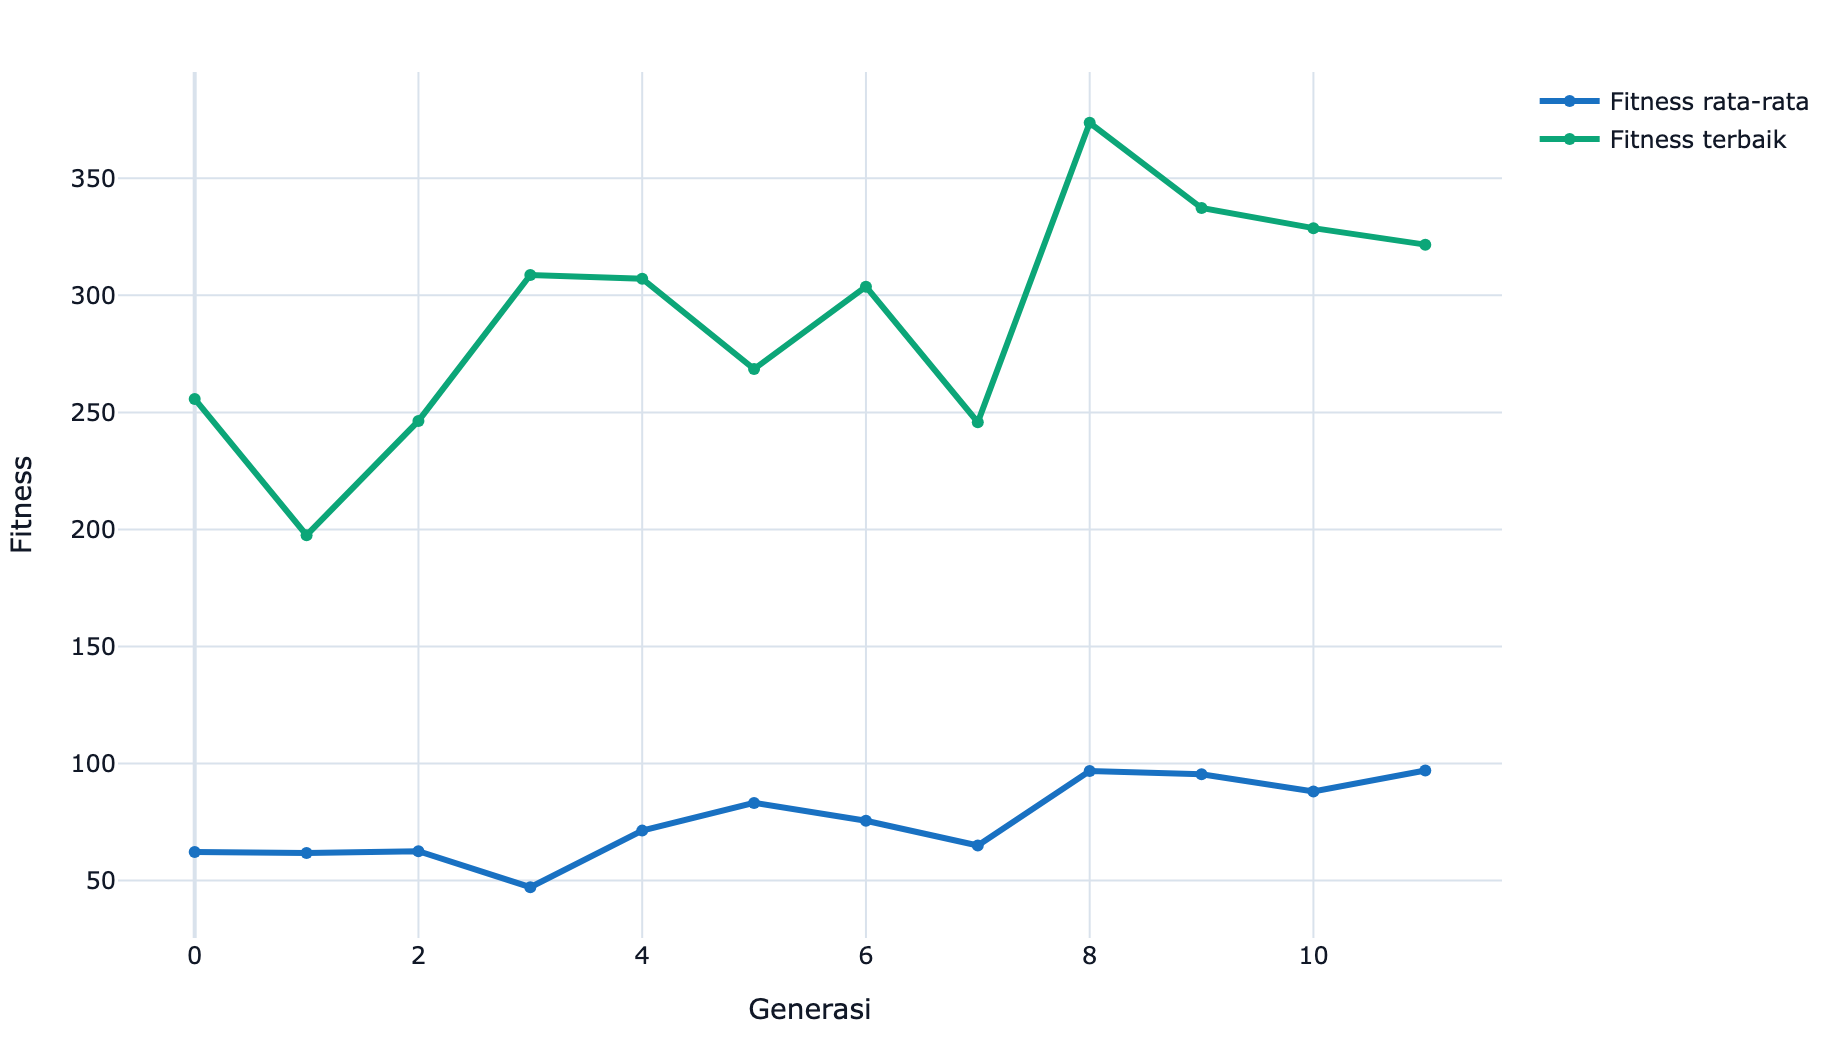
\includegraphics[width=0.49\textwidth]{figures/dashboard_fitness_history.png}
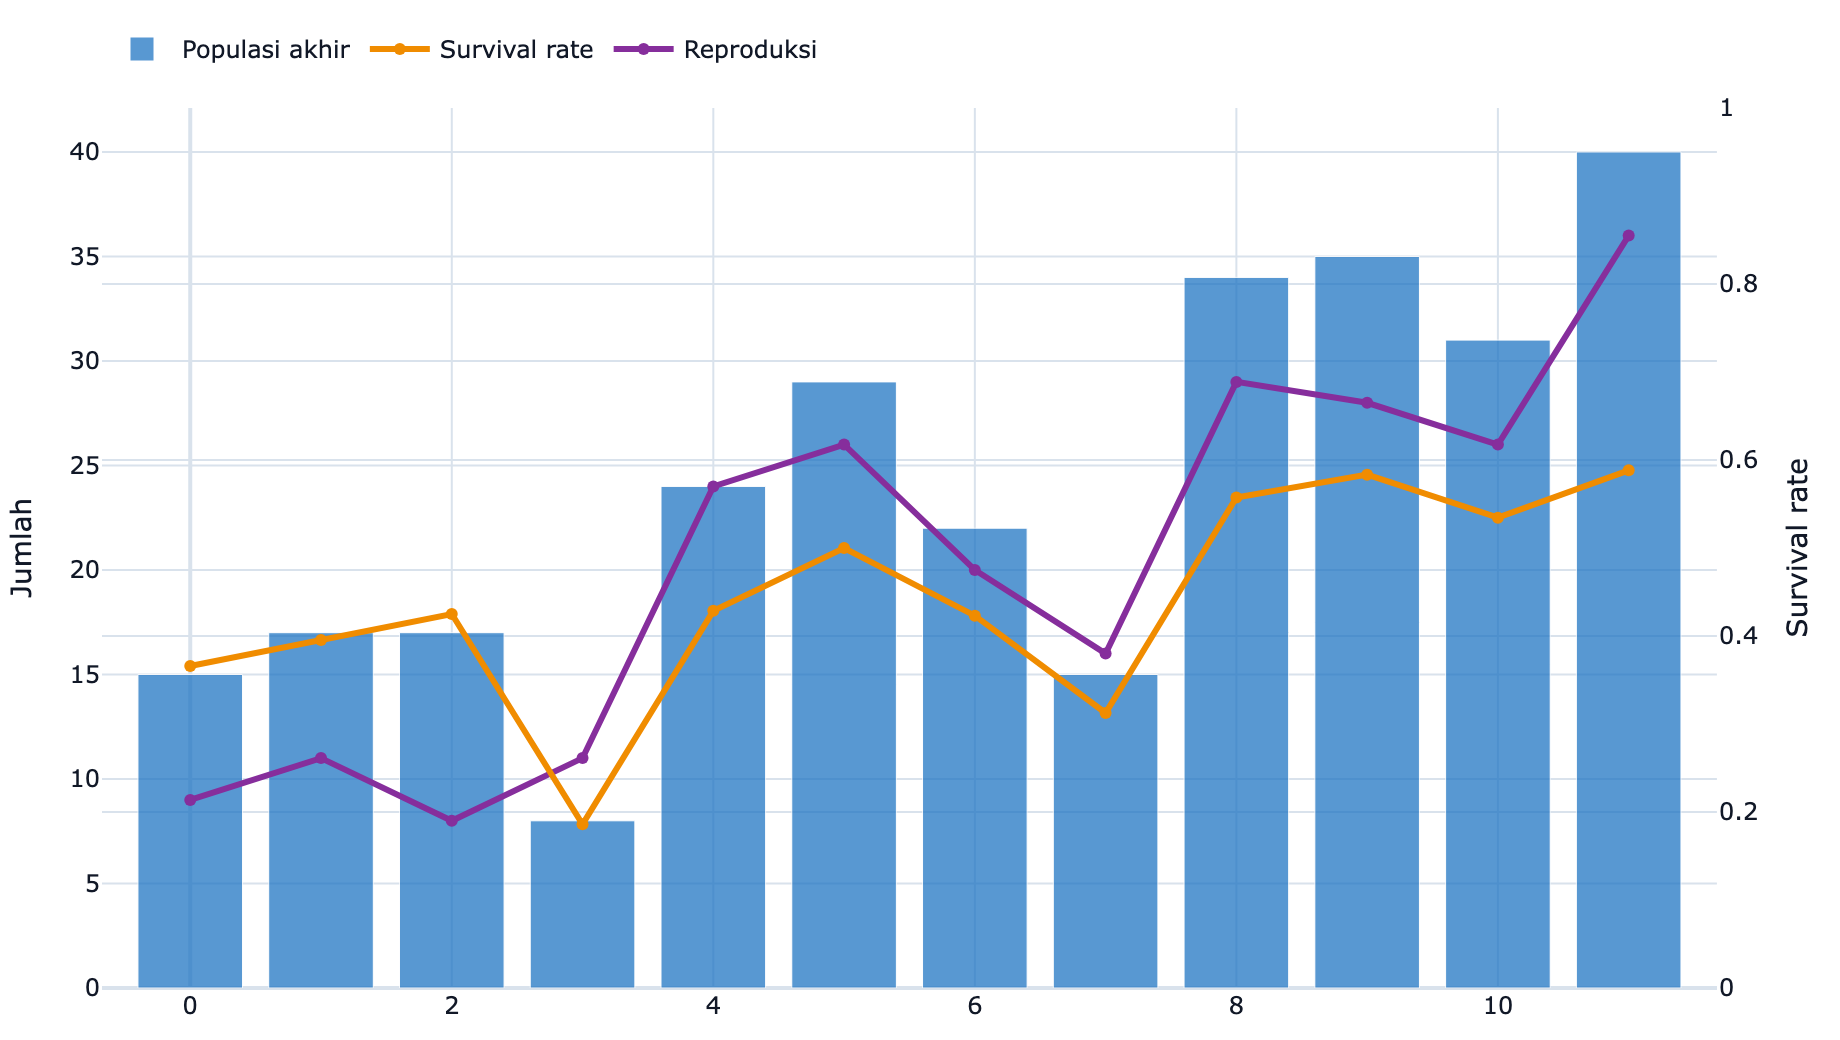
\includegraphics[width=0.49\textwidth]{figures/dashboard_population_history.png}
\caption{Dinamika temporal pada replikasi baseline, yaitu perkembangan fitness serta perubahan populasi, survival, dan reproduksi.}
\label{fig:hasil}
\end{figure}

Gambar \ref{fig:hasil} menunjukkan bahwa replikasi baseline mengalami kenaikan fitness dan fluktuasi survival-reproduksi yang tidak sepenuhnya linier. Pada agregasi lintas skenario, fitness akhir tertinggi tetap muncul pada eksplorasi tinggi, disusul hazard rendah dan baseline. Namun, urutan ini tidak dapat dibaca hanya sebagai ``semakin tinggi semakin baik'' karena setiap skenario mengubah tekanan ekologis. Eksplorasi tinggi menghasilkan makanan dan reproduksi paling banyak, tetapi simpangan bakunya juga terbesar, sedangkan hazard rendah membuat lingkungan lebih mudah dan baseline lebih seimbang dari sisi kenaikan fitness serta stabilitas.

\subsection{Efek Mutasi dan Tekanan Bahaya}
Efek mutasi terlihat jelas. Mutasi rendah menghasilkan fitness akhir 77,46 dan $\Delta F$ hanya 1,66. Artinya, populasi relatif stabil tetapi lambat menghasilkan variasi yang cukup untuk memperbaiki performa. Mutasi tinggi sedikit lebih baik, dengan fitness 79,86 dan $\Delta F$ 9,97, tetapi survival turun menjadi 0,53 dan paparan bahaya naik menjadi 124,67. Secara biologis, ini mencerminkan trade-off klasik, yaitu variasi diperlukan untuk adaptasi, tetapi mutasi berlebihan dapat merusak kombinasi sifat dan kebijakan yang sudah menguntungkan.

Tekanan bahaya juga memengaruhi hasil. Hazard rendah menghasilkan fitness 96,75, reproduksi 44,67, dan makanan 179,00. Lingkungan yang lebih aman memungkinkan agen mengalokasikan energi untuk foraging dan reproduksi. Sebaliknya, hazard tinggi menurunkan fitness menjadi 70,12, survival menjadi 0,52, dan makanan menjadi 108,00, meskipun $\Delta F$ masih 22,04. Interpretasinya, tekanan kuat masih dapat menyeleksi individu yang lebih baik daripada generasi awal, tetapi biaya ekologisnya besar, yaitu lebih banyak energi hilang, lebih banyak agen mati, dan ruang untuk reproduksi mengecil.

\subsection{Efek Eksplorasi}
Eksplorasi memberikan dampak paling menarik. Tanpa eksplorasi, fitness akhir hanya 76,08, reproduksi 9,00, makanan 82,67, dan Q-state 3489,50. Agen cenderung mengeksploitasi nilai awal atau kebijakan yang sempit sehingga peluang menemukan strategi makan dan reproduksi menurun. Eksplorasi tinggi menghasilkan fitness tertinggi, 100,04, reproduksi 51,33, makanan 223,00, dan Q-state 6523,11. Namun, simpangan baku 22,22 menunjukkan hasil lebih tidak stabil antar seed. Dalam konteks RL, eksplorasi memperluas pengalaman, sedangkan dalam konteks biologi, perilaku eksploratif dapat membuka akses sumber daya dan pasangan, tetapi juga meningkatkan risiko.

\subsection{Perubahan Sifat Populasi}
Perubahan sifat pada generasi akhir mendukung interpretasi bahwa fitness tidak ditentukan oleh trait saja. Baseline memiliki \textit{speed} 1,59, \textit{endurance} 1,31, \textit{foraging} 1,44, dan \textit{reproduction} 0,48. Hazard tinggi mempertahankan \textit{speed} dan \textit{endurance} relatif tinggi, sedangkan eksplorasi tinggi unggul pada Q-state dan makanan. Artinya, performa muncul dari kombinasi sifat bawaan, pengalaman state--aksi, dan tekanan lingkungan.

\begin{table}[h]
\centering
\caption{Rata-rata sifat biologis pada generasi akhir.}
\label{tab:sifat}
\begin{tabular}{lrrrr}
\toprule
Skenario & Speed & Endurance & Foraging & Reproduction \\
\midrule
Baseline & 1,59 & 1,31 & 1,44 & 0,48 \\
Mutasi rendah & 1,43 & 1,37 & 1,43 & 0,50 \\
Mutasi tinggi & 1,61 & 1,47 & 1,46 & 0,46 \\
Hazard rendah & 1,41 & 1,30 & 1,39 & 0,49 \\
Hazard tinggi & 1,61 & 1,42 & 1,42 & 0,44 \\
Tanpa eksplorasi & 1,45 & 1,28 & 1,50 & 0,50 \\
Eksplorasi tinggi & 1,44 & 1,39 & 1,42 & 0,47 \\
\bottomrule
\end{tabular}
\end{table}

Tabel \ref{tab:sifat} memperlihatkan bahwa perubahan sifat tidak selalu searah dengan fitness. Tanpa eksplorasi memiliki \textit{foraging} tertinggi, 1,50, tetapi makanan yang dimakan justru paling rendah, 82,67. Sebaliknya, eksplorasi tinggi mencapai 6523,11 Q-state dan makanan terbanyak. Ini menunjukkan bahwa trait yang tampak menguntungkan perlu didukung kebijakan perilaku yang kaya pengalaman, sedangkan Q-table menjadi perantara antara sifat bawaan dan keberhasilan ekologis.

Secara kualitatif, hasil simulasi menunjukkan tiga mekanisme adaptasi. Pertama, pembelajaran individual memperbaiki respons agen terhadap makanan, bahaya, dan pasangan. Kedua, seleksi antargenerasi menaikkan peluang sifat dan Q-table dari agen berfitness tinggi untuk diwariskan. Ketiga, mutasi menjaga keragaman sehingga populasi tidak terkunci pada kombinasi sifat awal. Ketiga mekanisme ini saling bergantung. Tanpa eksplorasi, agen tidak cukup belajar, tanpa mutasi, variasi melemah, dan tanpa tekanan seleksi, reproduksi tidak membedakan individu yang efektif dan tidak efektif.

\subsection{Keterbatasan Interpretasi}
Interpretasi hasil dibatasi oleh empat hal. Pertama, fitness adalah pendekatan komputasional yang mencampur reward, umur, makanan, reproduksi, dan bahaya, bukan fitness biologis yang sebenarnya. Kedua, Q-table diwariskan melalui crossover sehingga sebagian pengalaman induk diterima langsung oleh keturunan, yaitu asumsi model, bukan analogi biologis langsung. Ketiga, eksperimen hanya memakai tiga seed sehingga hasil perlu dibaca sebagai bukti awal. Keempat, performa tidak cukup dijelaskan oleh fitness akhir saja, yaitu $\Delta F$, survival rate, reproduksi, makanan, paparan bahaya, dan Q-state harus dibaca bersama.

Secara keseluruhan, hasil mendukung hipotesis bahwa adaptasi terbaik muncul dari kombinasi seimbang antara pembelajaran, variasi, dan tekanan seleksi. Lingkungan terlalu aman menaikkan reproduksi tetapi tidak selalu memberi kenaikan relatif besar, sedangkan lingkungan terlalu berbahaya menyeleksi individu yang bertahan tetapi menekan populasi. Eksperimen lanjutan perlu menambah seed, membandingkan pewarisan trait saja dan Q-table saja, menguji sensitivitas bobot fitness, serta membandingkan diskretisasi state kasar, sedang, dan halus.

\section{Kesimpulan}
Penelitian ini menunjukkan bahwa simulasi RL Evolution Lab dapat digunakan untuk menguji hubungan antara Q-learning, seleksi alam, mutasi, dan tekanan lingkungan secara kuantitatif. Kontribusi objektifnya adalah kerangka eksperimen yang dapat dijalankan ulang, metrik populasi yang terukur, serta analisis pembanding antarparameter. Eksperimen mandiri menunjukkan bahwa eksplorasi tinggi dan hazard rendah menghasilkan fitness akhir tertinggi, sedangkan hazard tinggi dan tanpa eksplorasi menurunkan performa. Mutasi rendah terlalu lambat memperbaiki populasi, sedangkan mutasi tinggi meningkatkan variasi tetapi menambah risiko.

Hasil simulasi menunjukkan bahwa pembelajaran perilaku melalui Q-learning dapat memperkuat adaptasi populasi ketika didukung variasi genetik dan tekanan seleksi yang memadai. Namun, performa populasi tidak hanya ditentukan oleh fitness akhir, melainkan juga oleh stabilitas antar-seed, survival rate, reproduksi, paparan bahaya, dan luasnya eksplorasi state. Karena itu, model ini lebih tepat dipahami sebagai kerangka eksploratif untuk mempelajari interaksi learning--evolution daripada sebagai model biologis empiris.

Saran penelitian berikutnya adalah menjalankan lebih banyak seed, memperpanjang jumlah generasi, membandingkan SARSA atau Expected SARSA dengan Q-learning, menguji mode pewarisan Q-table, menguji sensitivitas bobot fitness, dan membandingkan diskretisasi state. Ablation study juga perlu mencakup evolusi tanpa RL dan RL tanpa pewarisan Q-table. Untuk lingkungan yang lebih kompleks, DQN, Policy Gradient, atau Actor-Critic dapat dipakai ketika state dibuat kontinu atau berdimensi tinggi. Uji statistik seperti interval kepercayaan, ANOVA, atau Kruskal--Wallis dapat ditambahkan untuk memperkuat klaim antarskenario.

\bibliographystyle{plainnat}
\bibliography{paper}

\end{document}
